% Options for packages loaded elsewhere
\PassOptionsToPackage{unicode}{hyperref}
\PassOptionsToPackage{hyphens}{url}
%
\documentclass[
]{article}
\usepackage{lmodern}
\usepackage{amsmath}
\usepackage{ifxetex,ifluatex}
\ifnum 0\ifxetex 1\fi\ifluatex 1\fi=0 % if pdftex
  \usepackage[T1]{fontenc}
  \usepackage[utf8]{inputenc}
  \usepackage{textcomp} % provide euro and other symbols
  \usepackage{amssymb}
\else % if luatex or xetex
  \usepackage{unicode-math}
  \defaultfontfeatures{Scale=MatchLowercase}
  \defaultfontfeatures[\rmfamily]{Ligatures=TeX,Scale=1}
\fi
% Use upquote if available, for straight quotes in verbatim environments
\IfFileExists{upquote.sty}{\usepackage{upquote}}{}
\IfFileExists{microtype.sty}{% use microtype if available
  \usepackage[]{microtype}
  \UseMicrotypeSet[protrusion]{basicmath} % disable protrusion for tt fonts
}{}
\makeatletter
\@ifundefined{KOMAClassName}{% if non-KOMA class
  \IfFileExists{parskip.sty}{%
    \usepackage{parskip}
  }{% else
    \setlength{\parindent}{0pt}
    \setlength{\parskip}{6pt plus 2pt minus 1pt}}
}{% if KOMA class
  \KOMAoptions{parskip=half}}
\makeatother
\usepackage{xcolor}
\IfFileExists{xurl.sty}{\usepackage{xurl}}{} % add URL line breaks if available
\IfFileExists{bookmark.sty}{\usepackage{bookmark}}{\usepackage{hyperref}}
\hypersetup{
  pdftitle={Supervised binary classification on heart disease},
  pdfauthor={Loïc Rakotoson},
  hidelinks,
  pdfcreator={LaTeX via pandoc}}
\urlstyle{same} % disable monospaced font for URLs
\usepackage[margin=1cm]{geometry}
\usepackage{color}
\usepackage{fancyvrb}
\newcommand{\VerbBar}{|}
\newcommand{\VERB}{\Verb[commandchars=\\\{\}]}
\DefineVerbatimEnvironment{Highlighting}{Verbatim}{commandchars=\\\{\}}
% Add ',fontsize=\small' for more characters per line
\usepackage{framed}
\definecolor{shadecolor}{RGB}{248,248,248}
\newenvironment{Shaded}{\begin{snugshade}}{\end{snugshade}}
\newcommand{\AlertTok}[1]{\textcolor[rgb]{0.94,0.16,0.16}{#1}}
\newcommand{\AnnotationTok}[1]{\textcolor[rgb]{0.56,0.35,0.01}{\textbf{\textit{#1}}}}
\newcommand{\AttributeTok}[1]{\textcolor[rgb]{0.77,0.63,0.00}{#1}}
\newcommand{\BaseNTok}[1]{\textcolor[rgb]{0.00,0.00,0.81}{#1}}
\newcommand{\BuiltInTok}[1]{#1}
\newcommand{\CharTok}[1]{\textcolor[rgb]{0.31,0.60,0.02}{#1}}
\newcommand{\CommentTok}[1]{\textcolor[rgb]{0.56,0.35,0.01}{\textit{#1}}}
\newcommand{\CommentVarTok}[1]{\textcolor[rgb]{0.56,0.35,0.01}{\textbf{\textit{#1}}}}
\newcommand{\ConstantTok}[1]{\textcolor[rgb]{0.00,0.00,0.00}{#1}}
\newcommand{\ControlFlowTok}[1]{\textcolor[rgb]{0.13,0.29,0.53}{\textbf{#1}}}
\newcommand{\DataTypeTok}[1]{\textcolor[rgb]{0.13,0.29,0.53}{#1}}
\newcommand{\DecValTok}[1]{\textcolor[rgb]{0.00,0.00,0.81}{#1}}
\newcommand{\DocumentationTok}[1]{\textcolor[rgb]{0.56,0.35,0.01}{\textbf{\textit{#1}}}}
\newcommand{\ErrorTok}[1]{\textcolor[rgb]{0.64,0.00,0.00}{\textbf{#1}}}
\newcommand{\ExtensionTok}[1]{#1}
\newcommand{\FloatTok}[1]{\textcolor[rgb]{0.00,0.00,0.81}{#1}}
\newcommand{\FunctionTok}[1]{\textcolor[rgb]{0.00,0.00,0.00}{#1}}
\newcommand{\ImportTok}[1]{#1}
\newcommand{\InformationTok}[1]{\textcolor[rgb]{0.56,0.35,0.01}{\textbf{\textit{#1}}}}
\newcommand{\KeywordTok}[1]{\textcolor[rgb]{0.13,0.29,0.53}{\textbf{#1}}}
\newcommand{\NormalTok}[1]{#1}
\newcommand{\OperatorTok}[1]{\textcolor[rgb]{0.81,0.36,0.00}{\textbf{#1}}}
\newcommand{\OtherTok}[1]{\textcolor[rgb]{0.56,0.35,0.01}{#1}}
\newcommand{\PreprocessorTok}[1]{\textcolor[rgb]{0.56,0.35,0.01}{\textit{#1}}}
\newcommand{\RegionMarkerTok}[1]{#1}
\newcommand{\SpecialCharTok}[1]{\textcolor[rgb]{0.00,0.00,0.00}{#1}}
\newcommand{\SpecialStringTok}[1]{\textcolor[rgb]{0.31,0.60,0.02}{#1}}
\newcommand{\StringTok}[1]{\textcolor[rgb]{0.31,0.60,0.02}{#1}}
\newcommand{\VariableTok}[1]{\textcolor[rgb]{0.00,0.00,0.00}{#1}}
\newcommand{\VerbatimStringTok}[1]{\textcolor[rgb]{0.31,0.60,0.02}{#1}}
\newcommand{\WarningTok}[1]{\textcolor[rgb]{0.56,0.35,0.01}{\textbf{\textit{#1}}}}
\usepackage{graphicx}
\makeatletter
\def\maxwidth{\ifdim\Gin@nat@width>\linewidth\linewidth\else\Gin@nat@width\fi}
\def\maxheight{\ifdim\Gin@nat@height>\textheight\textheight\else\Gin@nat@height\fi}
\makeatother
% Scale images if necessary, so that they will not overflow the page
% margins by default, and it is still possible to overwrite the defaults
% using explicit options in \includegraphics[width, height, ...]{}
\setkeys{Gin}{width=\maxwidth,height=\maxheight,keepaspectratio}
% Set default figure placement to htbp
\makeatletter
\def\fps@figure{htbp}
\makeatother
\setlength{\emergencystretch}{3em} % prevent overfull lines
\providecommand{\tightlist}{%
  \setlength{\itemsep}{0pt}\setlength{\parskip}{0pt}}
\setcounter{secnumdepth}{-\maxdimen} % remove section numbering
\usepackage{booktabs}
\usepackage{longtable}
\usepackage{array}
\usepackage{multirow}
\usepackage{wrapfig}
\usepackage{float}
\usepackage{colortbl}
\usepackage{pdflscape}
\usepackage{tabu}
\usepackage{threeparttable}
\usepackage{threeparttablex}
\usepackage[normalem]{ulem}
\usepackage{makecell}
\usepackage{xcolor}
\ifluatex
  \usepackage{selnolig}  % disable illegal ligatures
\fi

\title{Supervised binary classification on heart disease}
\author{Loïc Rakotoson}
\date{}

\begin{document}
\maketitle

\hypertarget{abstract}{%
\section{Abstract}\label{abstract}}

In this paper we seek to perform a supervised classification to predict
the presence of heart disease based on several patient measurements.\\
In the following, the classification models will be optimized with
respect to the F1 score and Recall. This choice is explained by the
counterparts of bad predictions. Indeed, it would be more tolerated to
have false positives than undetected sick patients. With equal F1
performance, the Recall will allow to decide between two algorithms.

\hypertarget{introduction}{%
\section{Introduction}\label{introduction}}

When importing the data, the types given in the documentation were kept.
However, some numerical variables were directly discretized based on
their description in the same documentation.\\
Below are the first lines of our data.

\begin{Shaded}
\begin{Highlighting}[]
\NormalTok{data }\OperatorTok{=}\NormalTok{ (}
\NormalTok{    pd.read\_csv(}
        \StringTok{\textquotesingle{}heart.dat\textquotesingle{}}\NormalTok{, header}\OperatorTok{=}\VariableTok{None}\NormalTok{, sep}\OperatorTok{=}\StringTok{\textquotesingle{}\textbackslash{}s+\textquotesingle{}}\NormalTok{, engine}\OperatorTok{=}\StringTok{\textquotesingle{}python\textquotesingle{}}\NormalTok{,}
\NormalTok{        dtype}\OperatorTok{=}\NormalTok{\{}
            \DecValTok{0}\NormalTok{: np.}\BuiltInTok{int}\NormalTok{, }\DecValTok{1}\NormalTok{: }\StringTok{\textquotesingle{}category\textquotesingle{}}\NormalTok{, }\DecValTok{2}\NormalTok{: }\StringTok{\textquotesingle{}category\textquotesingle{}}\NormalTok{,}
            \DecValTok{3}\NormalTok{: np.}\BuiltInTok{int}\NormalTok{, }\DecValTok{4}\NormalTok{: np.}\BuiltInTok{float}\NormalTok{, }\DecValTok{5}\NormalTok{: np.}\BuiltInTok{bool}\NormalTok{,}
            \DecValTok{6}\NormalTok{: }\StringTok{\textquotesingle{}category\textquotesingle{}}\NormalTok{, }\DecValTok{7}\NormalTok{: np.}\BuiltInTok{int}\NormalTok{, }\DecValTok{8}\NormalTok{: np.}\BuiltInTok{bool}\NormalTok{,}
            \DecValTok{9}\NormalTok{: np.}\BuiltInTok{float}\NormalTok{, }\DecValTok{10}\NormalTok{: }\StringTok{\textquotesingle{}category\textquotesingle{}}\NormalTok{, }\DecValTok{11}\NormalTok{: }\StringTok{\textquotesingle{}category\textquotesingle{}}\NormalTok{,}
            \DecValTok{12}\NormalTok{: }\StringTok{\textquotesingle{}category\textquotesingle{}}\NormalTok{, }\DecValTok{13}\NormalTok{: }\StringTok{\textquotesingle{}category\textquotesingle{}}
\NormalTok{        \}}
\NormalTok{    ).rename(columns}\OperatorTok{=}\NormalTok{\{}
        \DecValTok{0}\NormalTok{: }\StringTok{"age"}\NormalTok{, }\DecValTok{1}\NormalTok{: }\StringTok{"sex"}\NormalTok{, }\DecValTok{2}\NormalTok{: }\StringTok{"chest\_pain"}\NormalTok{,}
        \DecValTok{3}\NormalTok{: }\StringTok{"blood\_pressure"}\NormalTok{, }\DecValTok{4}\NormalTok{: }\StringTok{"cholesterol"}\NormalTok{,}
        \DecValTok{5}\NormalTok{: }\StringTok{"blood\_sugar"}\NormalTok{, }\DecValTok{6}\NormalTok{: }\StringTok{"electrocard"}\NormalTok{,}
        \DecValTok{7}\NormalTok{: }\StringTok{"heart\_rate"}\NormalTok{, }\DecValTok{8}\NormalTok{: }\StringTok{"angina"}\NormalTok{, }\DecValTok{9}\NormalTok{: }\StringTok{"oldpeak"}\NormalTok{,}
        \DecValTok{10}\NormalTok{: }\StringTok{"slope\_peak"}\NormalTok{, }\DecValTok{11}\NormalTok{: }\StringTok{"vessels"}\NormalTok{, }\DecValTok{12}\NormalTok{: }\StringTok{"thal"}\NormalTok{,}
        \DecValTok{13}\NormalTok{: }\StringTok{"target"}
\NormalTok{    \})}
\NormalTok{)}
\end{Highlighting}
\end{Shaded}

\begin{table}

\caption{\label{tab:unnamed-chunk-11}First rows of data}
\centering
\resizebox{\linewidth}{!}{
\begin{tabular}[t]{rllrrllrlrllll}
\toprule
age & sex & chest\_pain & blood\_pressure & cholesterol & blood\_sugar & electrocard & heart\_rate & angina & oldpeak & slope\_peak & vessels & thal & target\\
\midrule
\cellcolor{gray!6}{70} & \cellcolor{gray!6}{1.0} & \cellcolor{gray!6}{4.0} & \cellcolor{gray!6}{130} & \cellcolor{gray!6}{322} & \cellcolor{gray!6}{FALSE} & \cellcolor{gray!6}{2.0} & \cellcolor{gray!6}{109} & \cellcolor{gray!6}{FALSE} & \cellcolor{gray!6}{2.4} & \cellcolor{gray!6}{2.0} & \cellcolor{gray!6}{3.0} & \cellcolor{gray!6}{3.0} & \cellcolor{gray!6}{2}\\
67 & 0.0 & 3.0 & 115 & 564 & FALSE & 2.0 & 160 & FALSE & 1.6 & 2.0 & 0.0 & 7.0 & 1\\
\cellcolor{gray!6}{57} & \cellcolor{gray!6}{1.0} & \cellcolor{gray!6}{2.0} & \cellcolor{gray!6}{124} & \cellcolor{gray!6}{261} & \cellcolor{gray!6}{FALSE} & \cellcolor{gray!6}{0.0} & \cellcolor{gray!6}{141} & \cellcolor{gray!6}{FALSE} & \cellcolor{gray!6}{0.3} & \cellcolor{gray!6}{1.0} & \cellcolor{gray!6}{0.0} & \cellcolor{gray!6}{7.0} & \cellcolor{gray!6}{2}\\
64 & 1.0 & 4.0 & 128 & 263 & FALSE & 0.0 & 105 & TRUE & 0.2 & 2.0 & 1.0 & 7.0 & 1\\
\cellcolor{gray!6}{74} & \cellcolor{gray!6}{0.0} & \cellcolor{gray!6}{2.0} & \cellcolor{gray!6}{120} & \cellcolor{gray!6}{269} & \cellcolor{gray!6}{FALSE} & \cellcolor{gray!6}{2.0} & \cellcolor{gray!6}{121} & \cellcolor{gray!6}{TRUE} & \cellcolor{gray!6}{0.2} & \cellcolor{gray!6}{1.0} & \cellcolor{gray!6}{1.0} & \cellcolor{gray!6}{3.0} & \cellcolor{gray!6}{1}\\
\addlinespace
65 & 1.0 & 4.0 & 120 & 177 & FALSE & 0.0 & 140 & FALSE & 0.4 & 1.0 & 0.0 & 7.0 & 1\\
\bottomrule
\end{tabular}}
\end{table}

\hypertarget{exploratory-data-analysis}{%
\section{Exploratory data analysis}\label{exploratory-data-analysis}}

To perform the analysis, groups of columns were created according to
their type.

The purpose of this analysis is to understand the data and derive
information, including distributions, correlations and covariances.

\hypertarget{target-analysis}{%
\subsection{Target analysis}\label{target-analysis}}

We have a binary target variable (\texttt{1}: absence and \texttt{2}:
presence of heart disease).\\
We are not dealing with an unbalanced variable, so there will be no need
to perform over-under-sampling strategies.

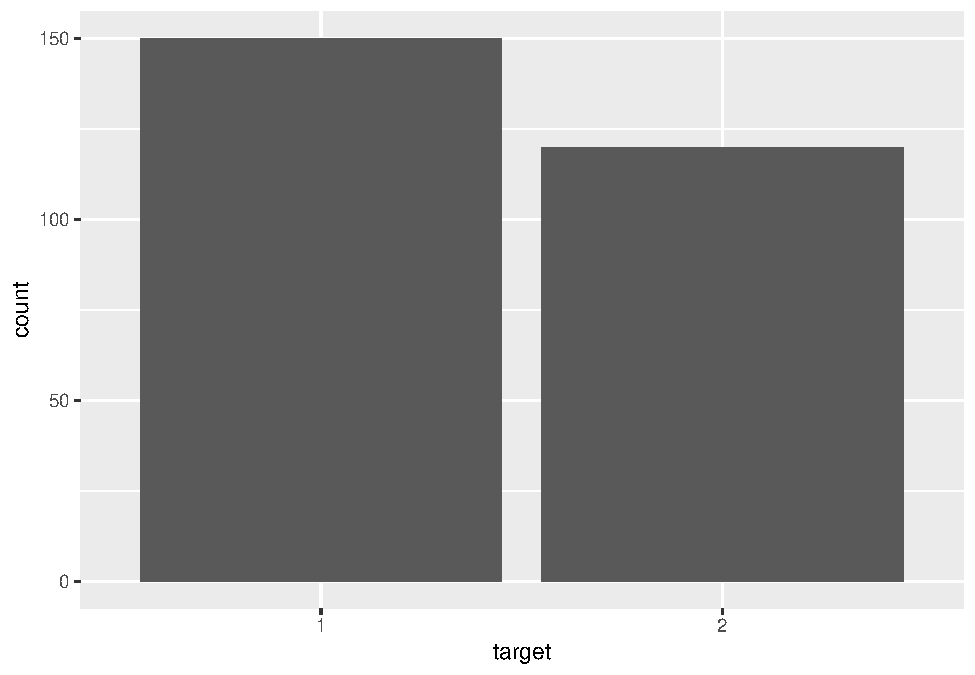
\includegraphics{hd_files/figure-latex/unnamed-chunk-13-1.pdf}

\hypertarget{analysis-of-qualitative-variables}{%
\subsection{Analysis of qualitative
variables}\label{analysis-of-qualitative-variables}}

\begin{itemize}
\tightlist
\item
  Each modality of the variable \texttt{blood\_sugar} has approximately
  the same target distribution. It does not vary the target.
\item
  The distribution of the target in vessels is the same when it is
  present. It can be transformed into a binary variable of presence or
  not. We observe the same phenomenon with \texttt{chest\_pain} where
  the \texttt{4} modality differs from the others which distribute the
  target in the same way.
\item
  There are only 2 people with the \texttt{1} modality of the
  \texttt{electrocard} variable, one of which is positive to the target.
  This modality has no variance. On the other hand, the ``0'' mode seems
  to discriminate the target. If the electrocard variable is used, it
  can be converted into binary by imputing the modality \texttt{1} and
  assigning the individual to one of the other modalities by means of a
  closest neighbor algorithm or by an average method for example.
\end{itemize}

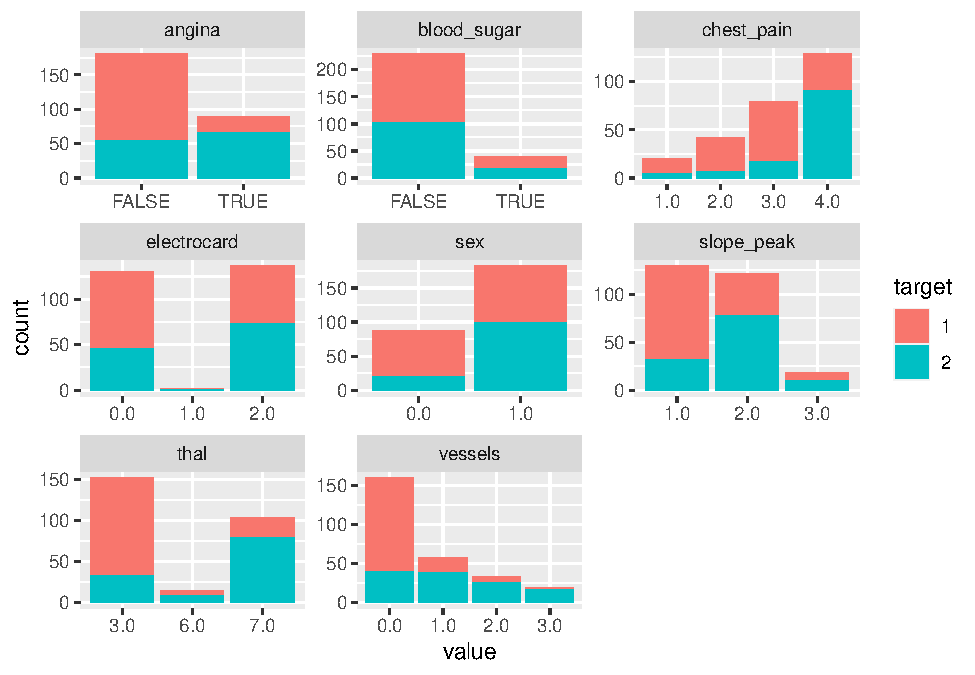
\includegraphics{hd_files/figure-latex/unnamed-chunk-14-1.pdf}

\begin{tabular}[t]{llllll}
\toprule
  &      age & blood\_pressure &  cholesterol &   heart\_rate &    oldpeak\\
\midrule
 & Min.   :29.00 & Min.   : 94.0 & Min.   :126.0 & Min.   : 71.0 & Min.   :0.00\\
 & 1st Qu.:48.00 & 1st Qu.:120.0 & 1st Qu.:213.0 & 1st Qu.:133.0 & 1st Qu.:0.00\\
 & Median :55.00 & Median :130.0 & Median :245.0 & Median :153.5 & Median :0.80\\
 & Mean   :54.43 & Mean   :131.3 & Mean   :249.7 & Mean   :149.7 & Mean   :1.05\\
 & 3rd Qu.:61.00 & 3rd Qu.:140.0 & 3rd Qu.:280.0 & 3rd Qu.:166.0 & 3rd Qu.:1.60\\
\addlinespace
 & Max.   :77.00 & Max.   :200.0 & Max.   :564.0 & Max.   :202.0 & Max.   :6.20\\
\bottomrule
\end{tabular}

\hypertarget{analysis-of-quantitative-variables}{%
\subsection{Analysis of quantitative
variables}\label{analysis-of-quantitative-variables}}

\begin{itemize}
\tightlist
\item
  The \texttt{blood\_presure} and \texttt{cholesterol} variables are
  each distributed approximately the same way with respect to the
  target, but with a slight shift.
\item
  The \texttt{age}, \texttt{heart\_rate} and \texttt{oldpeak} have a
  different distribution for each modality of the target.
\item
  The variable `oldpeak' has several outliers and there is a significant
  difference between the means and the medians for each of the target
  modalities. It is preferable to focus this variable on the median and
  reduce it between the 1st and 3rd quartile.
\end{itemize}

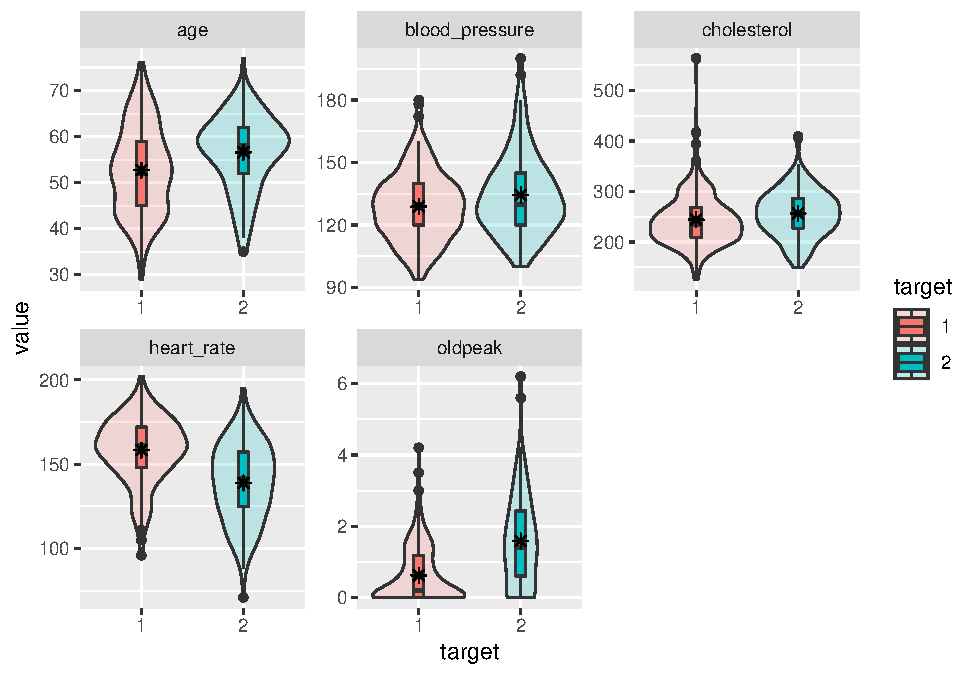
\includegraphics{hd_files/figure-latex/unnamed-chunk-17-1.pdf}

\newpage

The graph below shows the variable-variable relationships.\\
Note a certain negative correlation between the variable \texttt{age}
and \texttt{heart\_rate}.

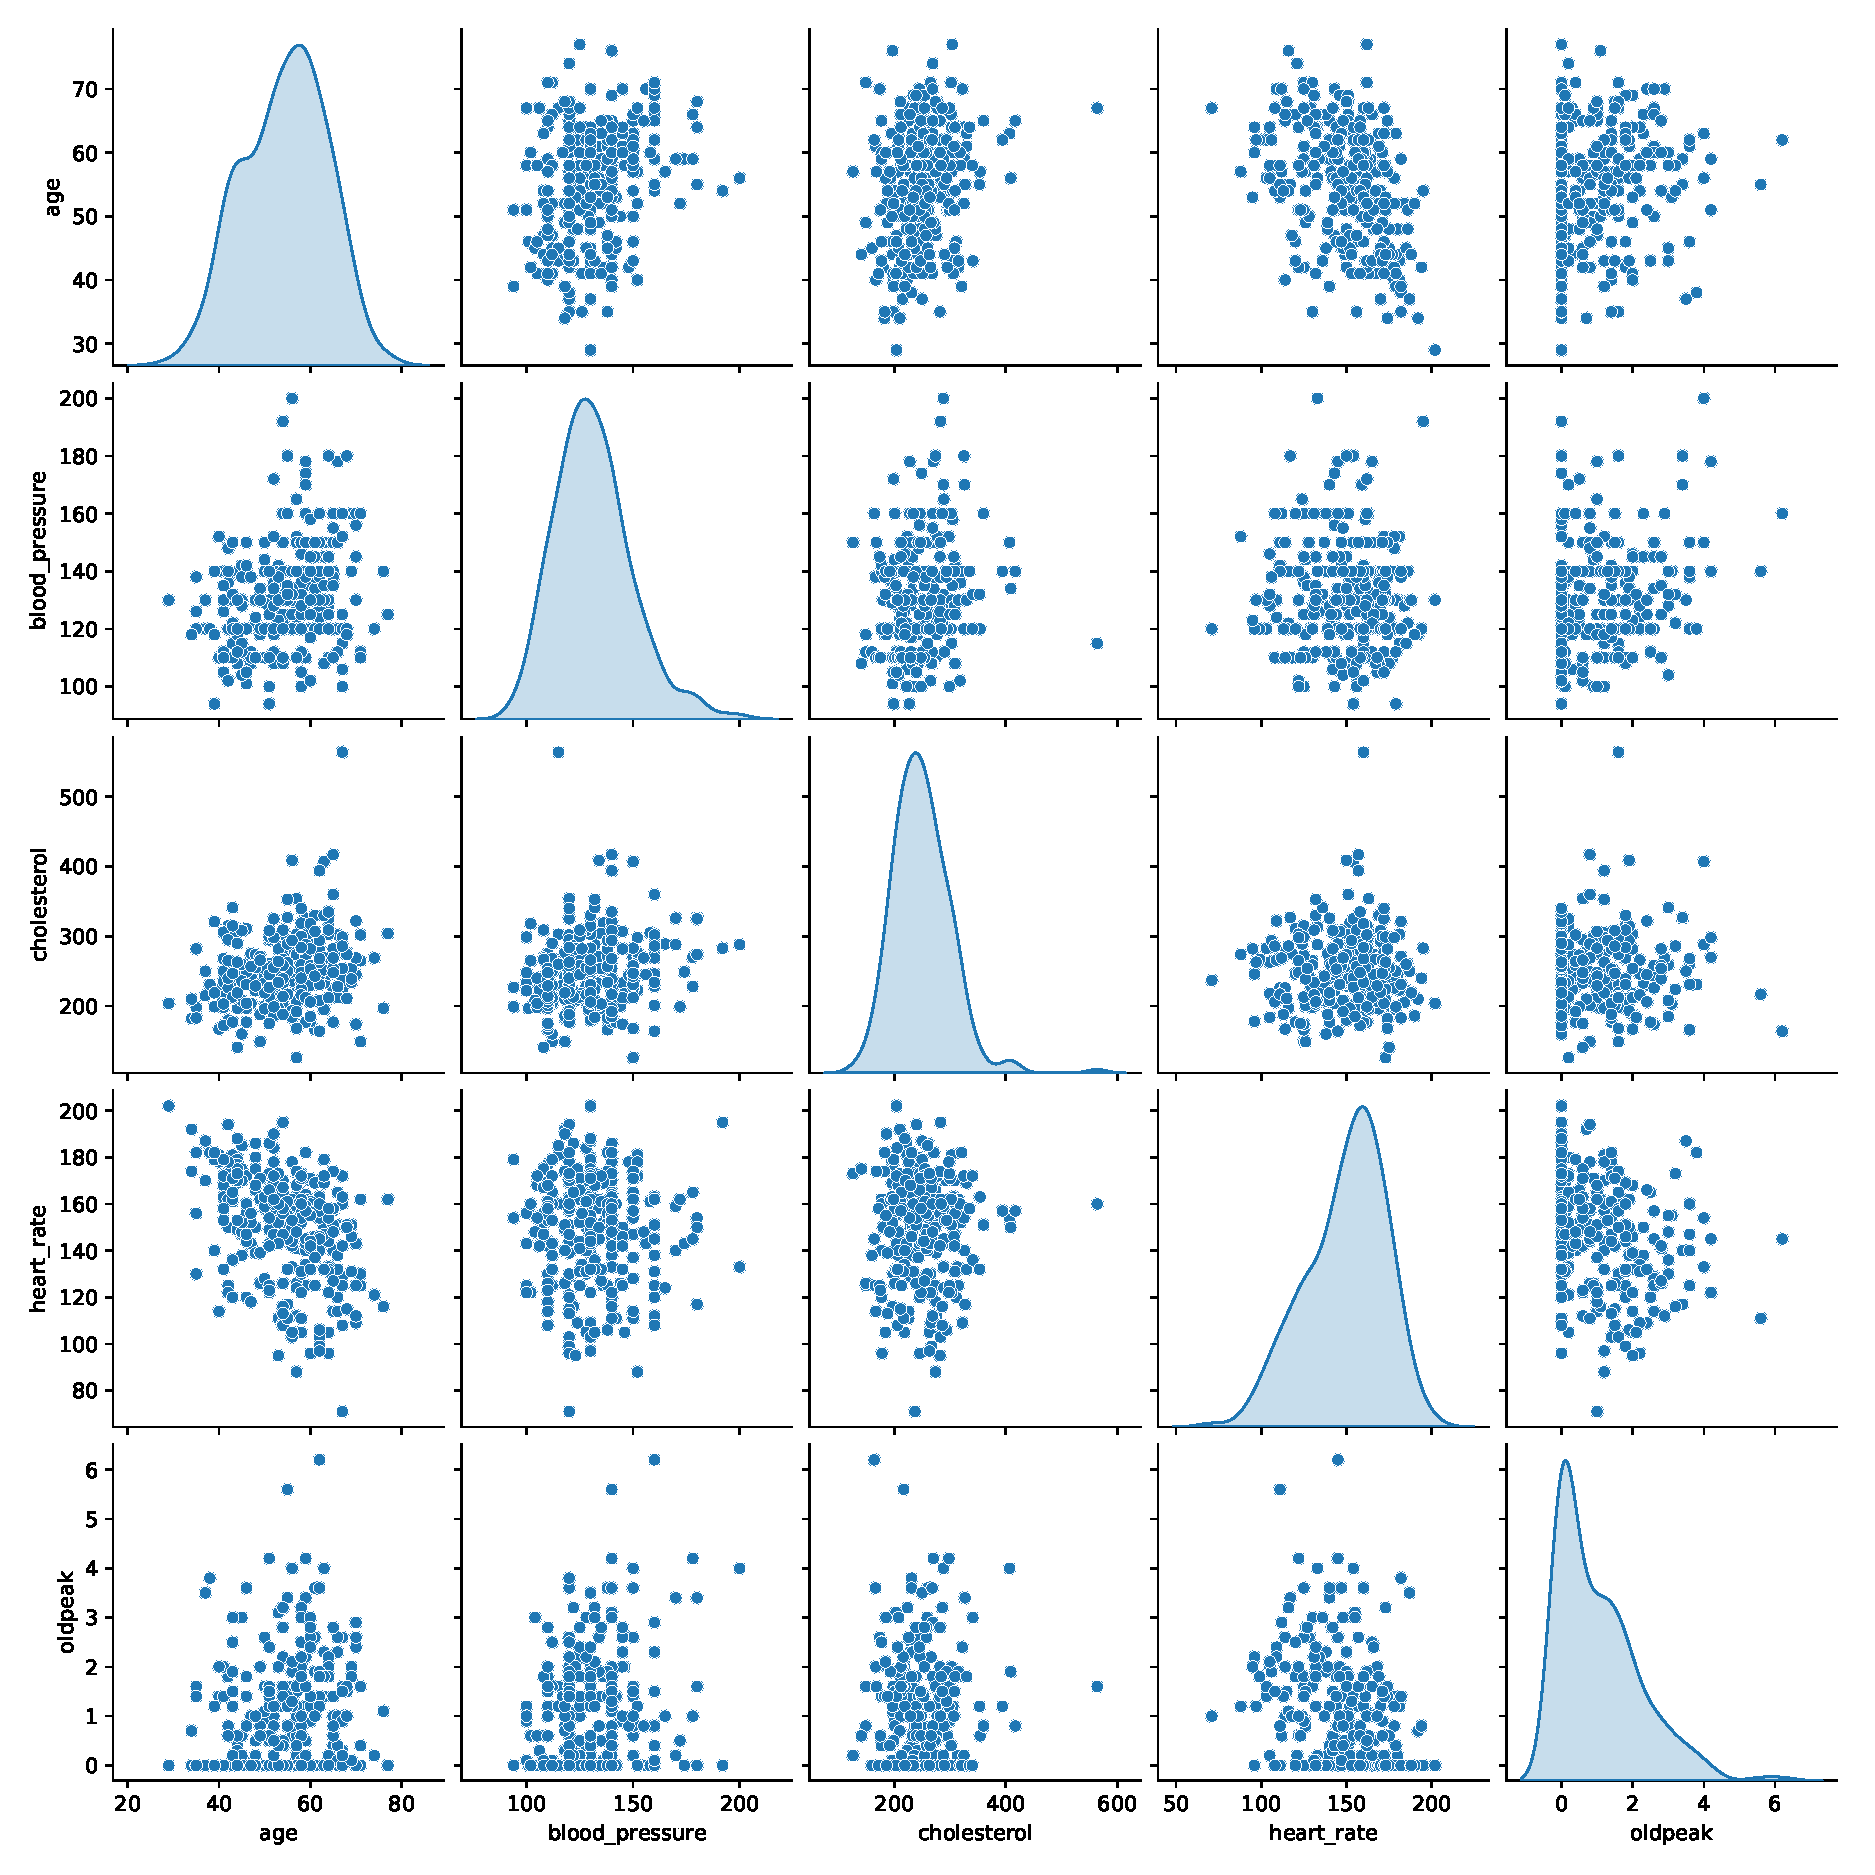
\includegraphics{hd_files/figure-latex/unnamed-chunk-18-1.pdf}

\hypertarget{preprocessing}{%
\section{Preprocessing}\label{preprocessing}}

Based on the exploratory analysis of the data, the pre-processing that
we will perform is as follows:

\begin{itemize}
\tightlist
\item
  Electrocard: Assigning the mode ``1'' to one of the other two with a
  ``KNNImputer'' and binarization.
\item
  \texttt{vessels} and \texttt{chest\_pain}: Grouping of variables
  according to the way the target is distributed and binarization
\item
  oldpeak: standardization with respect to the median
\item
  quantitative variables: standardization with respect to the mean
\end{itemize}

\begin{Shaded}
\begin{Highlighting}[]
\NormalTok{electropipe }\OperatorTok{=}\NormalTok{ Pipeline([(}\StringTok{\textquotesingle{}ls\textquotesingle{}}\NormalTok{, LessFrequent()), (}\StringTok{\textquotesingle{}scale\textquotesingle{}}\NormalTok{, MinMaxScaler()),}
\NormalTok{                        (}\StringTok{\textquotesingle{}inputer\textquotesingle{}}\NormalTok{, KNNImputer()),}
\NormalTok{                        (}\StringTok{\textquotesingle{}calib\textquotesingle{}}\NormalTok{, Binarizer(threshold}\OperatorTok{=}\FloatTok{.5}\NormalTok{))])}

\NormalTok{preprocess }\OperatorTok{=}\NormalTok{ ColumnTransformer(}
\NormalTok{    remainder}\OperatorTok{=}\StringTok{\textquotesingle{}passthrough\textquotesingle{}}\NormalTok{,}
\NormalTok{    transformers}\OperatorTok{=}\NormalTok{[(}\StringTok{\textquotesingle{}inp\textquotesingle{}}\NormalTok{, electropipe, [}\StringTok{\textquotesingle{}electrocard\textquotesingle{}}\NormalTok{]),}
\NormalTok{                  (}\StringTok{\textquotesingle{}topbin\textquotesingle{}}\NormalTok{, IsTop(), [}\StringTok{\textquotesingle{}vessels\textquotesingle{}}\NormalTok{, }\StringTok{\textquotesingle{}chest\_pain\textquotesingle{}}\NormalTok{]),}
\NormalTok{                  (}\StringTok{\textquotesingle{}bin\textquotesingle{}}\NormalTok{, Binarizer(), [}\StringTok{\textquotesingle{}angina\textquotesingle{}}\NormalTok{, }\StringTok{\textquotesingle{}blood\_sugar\textquotesingle{}}\NormalTok{, }\StringTok{\textquotesingle{}sex\textquotesingle{}}\NormalTok{]),}
\NormalTok{                  (}\StringTok{\textquotesingle{}ordinal\textquotesingle{}}\NormalTok{, OrdinalEncoder(), [}\StringTok{\textquotesingle{}slope\_peak\textquotesingle{}}\NormalTok{]),}
\NormalTok{                  (}\StringTok{\textquotesingle{}onehot\textquotesingle{}}\NormalTok{, OneHotEncoder(drop}\OperatorTok{=}\StringTok{\textquotesingle{}first\textquotesingle{}}\NormalTok{), [}\StringTok{\textquotesingle{}thal\textquotesingle{}}\NormalTok{]),}
\NormalTok{                  (}\StringTok{\textquotesingle{}standard\textquotesingle{}}\NormalTok{, StandardScaler(), numerical[:}\OperatorTok{{-}}\DecValTok{1}\NormalTok{]),}
\NormalTok{                  (}\StringTok{\textquotesingle{}scaler\textquotesingle{}}\NormalTok{, RobustScaler(), [}\StringTok{\textquotesingle{}oldpeak\textquotesingle{}}\NormalTok{])])}

\NormalTok{label }\OperatorTok{=}\NormalTok{ LabelBinarizer()}
\end{Highlighting}
\end{Shaded}

The data is then separated into training and test sets.

\begin{Shaded}
\begin{Highlighting}[]
\NormalTok{x\_train, x\_test }\OperatorTok{=}\NormalTok{ train\_test\_split(data, test\_size}\OperatorTok{=}\FloatTok{.2}\NormalTok{, random\_state}\OperatorTok{=}\DecValTok{42069}\NormalTok{)}
\NormalTok{y\_train }\OperatorTok{=}\NormalTok{ label.fit\_transform(x\_train.pop(}\StringTok{\textquotesingle{}target\textquotesingle{}}\NormalTok{))}
\NormalTok{y\_test }\OperatorTok{=}\NormalTok{ label.transform(x\_test.pop(}\StringTok{\textquotesingle{}target\textquotesingle{}}\NormalTok{))}
\end{Highlighting}
\end{Shaded}

\begin{table}

\caption{\label{tab:unnamed-chunk-22}Preprocessed data}
\centering
\resizebox{\linewidth}{!}{
\begin{tabular}[t]{rrrrrrrrrrrrrrr}
\toprule
inp\_\_electrocard & topbin\_\_vessels & topbin\_\_chest\_pain & bin\_\_angina & bin\_\_blood\_sugar & bin\_\_sex & ordinal\_\_slope\_peak & onehot\_\_x0\_6.0 & onehot\_\_x0\_7.0 & standard\_\_age & standard\_\_blood\_pressure & standard\_\_cholesterol & standard\_\_heart\_rate & scaler\_\_oldpeak & target\\
\midrule
\cellcolor{gray!6}{1} & \cellcolor{gray!6}{0} & \cellcolor{gray!6}{0} & \cellcolor{gray!6}{1} & \cellcolor{gray!6}{0} & \cellcolor{gray!6}{1} & \cellcolor{gray!6}{0} & \cellcolor{gray!6}{0} & \cellcolor{gray!6}{0} & \cellcolor{gray!6}{-0.3986754} & \cellcolor{gray!6}{-0.3197880} & \cellcolor{gray!6}{-0.7046617} & \cellcolor{gray!6}{-1.0492113} & \cellcolor{gray!6}{0.3750} & \cellcolor{gray!6}{0}\\
1 & 0 & 1 & 1 & 0 & 1 & 1 & 0 & 0 & 1.3454033 & -1.7576357 & 0.8955578 & -1.0492113 & 0.0625 & 1\\
\cellcolor{gray!6}{1} & \cellcolor{gray!6}{0} & \cellcolor{gray!6}{1} & \cellcolor{gray!6}{0} & \cellcolor{gray!6}{0} & \cellcolor{gray!6}{1} & \cellcolor{gray!6}{0} & \cellcolor{gray!6}{0} & \cellcolor{gray!6}{0} & \cellcolor{gray!6}{-1.1617098} & \cellcolor{gray!6}{-1.1824966} & \cellcolor{gray!6}{-1.0023769} & \cellcolor{gray!6}{1.2032240} & \cellcolor{gray!6}{-0.5000} & \cellcolor{gray!6}{1}\\
1 & 0 & 0 & 0 & 1 & 0 & 0 & 0 & 0 & 0.3643590 & 0.3128650 & 1.2677018 & 0.1203224 & -0.5000 & 1\\
\cellcolor{gray!6}{0} & \cellcolor{gray!6}{1} & \cellcolor{gray!6}{0} & \cellcolor{gray!6}{0} & \cellcolor{gray!6}{0} & \cellcolor{gray!6}{1} & \cellcolor{gray!6}{2} & \cellcolor{gray!6}{0} & \cellcolor{gray!6}{1} & \cellcolor{gray!6}{-0.7256901} & \cellcolor{gray!6}{-1.1824966} & \cellcolor{gray!6}{-0.4069464} & \cellcolor{gray!6}{0.8133794} & \cellcolor{gray!6}{0.1250} & \cellcolor{gray!6}{1}\\
\addlinespace
0 & 1 & 0 & 0 & 0 & 1 & 0 & 0 & 0 & 0.1463492 & -0.6073575 & -0.2766960 & 1.2465400 & 0.0000 & 0\\
\bottomrule
\end{tabular}}
\end{table}

\hypertarget{modeling}{%
\section{Modeling}\label{modeling}}

\hypertarget{naive-benchmark}{%
\subsection{Naive Benchmark}\label{naive-benchmark}}

In the following we will perform a naive benchmark of the classical
models used for binary classification.\\
We will capture as score the f1, recall and accuracy.

We chose to optimize the first 3 algorithms as well as Adaboost which
stands out with a good recall score despite the low f1.

\begin{table}

\caption{\label{tab:unnamed-chunk-25}Naive benchmark results}
\centering
\begin{tabu} to \linewidth {>{\raggedright\arraybackslash}p{8cm}>{\raggedleft}X>{\raggedleft}X>{\raggedleft}X}
\toprule
model & accuracy & f1\_score & recall\\
\midrule
Logistic Regression & 0.9074074 & 0.8979592 & 0.9166667\\
SGD Classifier & 0.9074074 & 0.8936170 & 0.8750000\\
Neural Net & 0.8888889 & 0.8800000 & 0.9166667\\
Naive Bayes & 0.8888889 & 0.8800000 & 0.9166667\\
KNN & 0.8888889 & 0.8695652 & 0.8333333\\
\addlinespace
Gaussian Process & 0.8703704 & 0.8571429 & 0.8750000\\
Random Forest & 0.8703704 & 0.8510638 & 0.8333333\\
QDA & 0.8703704 & 0.8510638 & 0.8333333\\
AdaBoost & 0.8333333 & 0.8235294 & 0.8750000\\
Linear SVM & 0.8518519 & 0.8181818 & 0.7500000\\
\addlinespace
Decision Tree & 0.8518519 & 0.8181818 & 0.7500000\\
RBF SVM & 0.5740741 & 0.0800000 & 0.0416667\\
\bottomrule
\end{tabu}
\end{table}

\hypertarget{optimization}{%
\subsection{Optimization}\label{optimization}}

For the optimization, we will choose the strategy of ``Nested Grid
Search Cross Validation'' which consists in having 2 cross validations:

\begin{itemize}
\tightlist
\item
  A first one for the search of the best hyperparameters in a grid using
  a 4-fold KFold.
\item
  A second one to obtain the score of the best hyperparameters chosen
  using a 6 Fold KFold, thus data not used for training.
\end{itemize}

We will also introduce the neighbor parameter to impute it even if with
2 individuals, the chance of its presence in a Fold is low.

\begin{Shaded}
\begin{Highlighting}[]
\NormalTok{cv\_inner }\OperatorTok{=}\NormalTok{ KFold(n\_splits }\OperatorTok{=} \DecValTok{4}\NormalTok{, shuffle }\OperatorTok{=} \VariableTok{True}\NormalTok{, random\_state }\OperatorTok{=} \DecValTok{42069}\NormalTok{)}
\NormalTok{cv\_outer }\OperatorTok{=}\NormalTok{ KFold(n\_splits }\OperatorTok{=} \DecValTok{6}\NormalTok{, shuffle }\OperatorTok{=} \VariableTok{True}\NormalTok{, random\_state }\OperatorTok{=} \DecValTok{42069}\NormalTok{)}
\end{Highlighting}
\end{Shaded}

\hypertarget{logistic-regression}{%
\subsubsection{Logistic Regression}\label{logistic-regression}}

As our dataset is quite light, it is interesting to see the absence or
presence of regularization (l1 or l2).\\
The \texttt{liblinear} solver performs well on small datasets, while the
`lbfgs' solver theoretically handles well the absence of
regularization.\\
Finally, the last parameter to be optimized is the number of iterations.
We will choose the 3 ``classical'' values.

\begin{Shaded}
\begin{Highlighting}[]
\NormalTok{model1 }\OperatorTok{=}\NormalTok{ Pipeline([}
\NormalTok{    (}\StringTok{\textquotesingle{}preprocess\textquotesingle{}}\NormalTok{, preprocess),}
\NormalTok{    (}\StringTok{\textquotesingle{}clf\textquotesingle{}}\NormalTok{, LogisticRegression())}
\NormalTok{])}

\NormalTok{params }\OperatorTok{=}\NormalTok{ \{}
    \StringTok{\textquotesingle{}preprocess\_\_inp\_\_inputer\_\_n\_neighbors\textquotesingle{}}\NormalTok{: np.arange(}\DecValTok{3}\NormalTok{, }\DecValTok{10}\NormalTok{, }\DecValTok{2}\NormalTok{),}
    \StringTok{\textquotesingle{}clf\_\_penalty\textquotesingle{}}\NormalTok{: [}\StringTok{\textquotesingle{}l1\textquotesingle{}}\NormalTok{, }\StringTok{\textquotesingle{}l2\textquotesingle{}}\NormalTok{, }\StringTok{\textquotesingle{}none\textquotesingle{}}\NormalTok{],}
    \StringTok{\textquotesingle{}clf\_\_solver\textquotesingle{}}\NormalTok{: [}\StringTok{\textquotesingle{}liblinear\textquotesingle{}}\NormalTok{, }\StringTok{\textquotesingle{}lbfgs\textquotesingle{}}\NormalTok{],}
    \StringTok{\textquotesingle{}clf\_\_max\_iter\textquotesingle{}}\NormalTok{: [}\FloatTok{1e2}\NormalTok{, }\FloatTok{1.5e2}\NormalTok{, }\FloatTok{1e3}\NormalTok{]}
\NormalTok{\}}

\NormalTok{result1, best1 }\OperatorTok{=}\NormalTok{ nestedCV(}
\NormalTok{    model1, params, x\_train, y\_train,}
\NormalTok{    cv\_inner, cv\_outer, name }\OperatorTok{=} \StringTok{"Logistic Regression"}\NormalTok{,}
\NormalTok{)}
\end{Highlighting}
\end{Shaded}

\begin{table}

\caption{\label{tab:unnamed-chunk-29}Best hyperparameters for logistic regression}
\centering
\resizebox{\linewidth}{!}{
\begin{tabular}[t]{rllrlrrrrr}
\toprule
preprocess\_\_inp\_\_inputer\_\_n\_neighbors & clf\_\_penalty & clf\_\_solver & clf\_\_max\_iter & name & f1\_score & inner\_score & recall & accuracy & count\\
\midrule
\cellcolor{gray!6}{3} & \cellcolor{gray!6}{l1} & \cellcolor{gray!6}{liblinear} & \cellcolor{gray!6}{100} & \cellcolor{gray!6}{Logistic Regression} & \cellcolor{gray!6}{0.7815603} & \cellcolor{gray!6}{0.8087427} & \cellcolor{gray!6}{0.8065476} & \cellcolor{gray!6}{0.8240741} & \cellcolor{gray!6}{3}\\
3 & l2 & lbfgs & 100 & Logistic Regression & 0.8279112 & 0.8152803 & 0.7426901 & 0.8518519 & 3\\
\bottomrule
\end{tabular}}
\end{table}

\hypertarget{naive-bayes}{%
\subsubsection{Naive Bayes}\label{naive-bayes}}

The only hyperparameter to be optimized here is the variance share of
the data for the variance update: \texttt{var\_smoothing}.\\
We will choose a grid of 50 parameters between 1 and 10 -20 .

\begin{Shaded}
\begin{Highlighting}[]
\NormalTok{model2 }\OperatorTok{=}\NormalTok{ Pipeline([}
\NormalTok{    (}\StringTok{\textquotesingle{}preprocess\textquotesingle{}}\NormalTok{, preprocess),}
\NormalTok{    (}\StringTok{\textquotesingle{}clf\textquotesingle{}}\NormalTok{, GaussianNB())}
\NormalTok{])}

\NormalTok{params }\OperatorTok{=}\NormalTok{ \{}
    \StringTok{\textquotesingle{}preprocess\_\_inp\_\_inputer\_\_n\_neighbors\textquotesingle{}}\NormalTok{: np.arange(}\DecValTok{3}\NormalTok{, }\DecValTok{10}\NormalTok{, }\DecValTok{2}\NormalTok{),}
    \StringTok{\textquotesingle{}clf\_\_var\_smoothing\textquotesingle{}}\NormalTok{: np.logspace(}\DecValTok{0}\NormalTok{, }\OperatorTok{{-}}\DecValTok{20}\NormalTok{, num }\OperatorTok{=} \DecValTok{50}\NormalTok{)}
\NormalTok{\}}

\NormalTok{result2, best2 }\OperatorTok{=}\NormalTok{ nestedCV(}
\NormalTok{    model2, params, x\_train, y\_train,}
\NormalTok{    cv\_inner, cv\_outer, name }\OperatorTok{=} \StringTok{"Naive Bayes"}
\NormalTok{)}
\end{Highlighting}
\end{Shaded}

\begin{table}

\caption{\label{tab:unnamed-chunk-32}Naive Bayes best parameters}
\centering
\resizebox{\linewidth}{!}{
\begin{tabular}[t]{rrlrrrrr}
\toprule
preprocess\_\_inp\_\_inputer\_\_n\_neighbors & clf\_\_var\_smoothing & name & f1\_score & inner\_score & recall & accuracy & count\\
\midrule
\cellcolor{gray!6}{3} & \cellcolor{gray!6}{0.0232995} & \cellcolor{gray!6}{Naive Bayes} & \cellcolor{gray!6}{0.8421053} & \cellcolor{gray!6}{0.8285947} & \cellcolor{gray!6}{0.8000000} & \cellcolor{gray!6}{0.8333333} & \cellcolor{gray!6}{1}\\
3 & 0.0596362 & Naive Bayes & 0.7992342 & 0.8205153 & 0.7652778 & 0.8425926 & 3\\
\cellcolor{gray!6}{3} & \cellcolor{gray!6}{0.1526418} & \cellcolor{gray!6}{Naive Bayes} & \cellcolor{gray!6}{0.8506944} & \cellcolor{gray!6}{0.7978685} & \cellcolor{gray!6}{0.8853383} & \cellcolor{gray!6}{0.8611111} & \cellcolor{gray!6}{2}\\
\bottomrule
\end{tabular}}
\end{table}

\hypertarget{neural-network}{%
\subsubsection{Neural network}\label{neural-network}}

Multilayer perceptrons are optimized here.\\
The hyperparameters that we will optimize are:

\begin{itemize}
\tightlist
\item
  The size of the hidden layers
\item
  The activation functions, \texttt{logistic} and \texttt{tanh} because
  our data is binary data, \texttt{relu} because all data is positive
  values.
\item
  The optimizer, \texttt{sgd} classic, \texttt{adam} the \texttt{best}
  for now and \texttt{lbfgs} for small data sizes
\item
  The behavior of \(\alpha\) that decreases either as a function of the
  steps or as a function of the loss function.
\end{itemize}

We will activate the \texttt{early\ stopping} to avoid overfitting and
we will allow ourselves to have a fairly high number of iterations.

\begin{Shaded}
\begin{Highlighting}[]
\NormalTok{model3 }\OperatorTok{=}\NormalTok{ Pipeline([}
\NormalTok{    (}\StringTok{\textquotesingle{}preprocess\textquotesingle{}}\NormalTok{, preprocess),}
\NormalTok{    (}\StringTok{\textquotesingle{}clf\textquotesingle{}}\NormalTok{, MLPClassifier(}
\NormalTok{        batch\_size }\OperatorTok{=} \DecValTok{200}\NormalTok{,}
\NormalTok{        learning\_rate\_init }\OperatorTok{=} \FloatTok{1e{-}3}\NormalTok{,}
\NormalTok{        max\_iter }\OperatorTok{=} \FloatTok{1e3}\NormalTok{,}
\NormalTok{        early\_stopping }\OperatorTok{=} \VariableTok{True}\NormalTok{,}
\NormalTok{        n\_iter\_no\_change }\OperatorTok{=} \DecValTok{15}
\NormalTok{    ))}
\NormalTok{])}

\NormalTok{params }\OperatorTok{=}\NormalTok{ \{}
    \StringTok{\textquotesingle{}clf\_\_hidden\_layer\_sizes\textquotesingle{}}\NormalTok{: [}
\NormalTok{        (}\DecValTok{10}\NormalTok{,), (}\DecValTok{50}\NormalTok{,), (}\DecValTok{100}\NormalTok{,), (}\DecValTok{150}\NormalTok{,), (}\DecValTok{200}\NormalTok{,)],}
    \StringTok{\textquotesingle{}clf\_\_activation\textquotesingle{}}\NormalTok{: [}\StringTok{\textquotesingle{}logistic\textquotesingle{}}\NormalTok{, }\StringTok{\textquotesingle{}relu\textquotesingle{}}\NormalTok{, }\StringTok{\textquotesingle{}tanh\textquotesingle{}}\NormalTok{],}
    \StringTok{\textquotesingle{}clf\_\_solver\textquotesingle{}}\NormalTok{: [}\StringTok{\textquotesingle{}lbfgs\textquotesingle{}}\NormalTok{, }\StringTok{\textquotesingle{}adam\textquotesingle{}}\NormalTok{, }\StringTok{\textquotesingle{}sgd\textquotesingle{}}\NormalTok{],}
    \StringTok{\textquotesingle{}clf\_\_learning\_rate\textquotesingle{}}\NormalTok{: [}\StringTok{\textquotesingle{}invscaling\textquotesingle{}}\NormalTok{, }\StringTok{\textquotesingle{}adaptive\textquotesingle{}}\NormalTok{]}
\NormalTok{\}}

\NormalTok{result3, best3 }\OperatorTok{=}\NormalTok{ nestedCV(}
\NormalTok{    model3, params, x\_train, y\_train,}
\NormalTok{    cv\_inner, cv\_outer, name }\OperatorTok{=} \StringTok{"Neural Network"}
\NormalTok{)}
\end{Highlighting}
\end{Shaded}

\begin{table}

\caption{\label{tab:unnamed-chunk-35}Multilayer Perceptron best parameters}
\centering
\resizebox{\linewidth}{!}{
\begin{tabular}[t]{rllllrrrrr}
\toprule
clf\_\_hidden\_layer\_sizes & clf\_\_activation & clf\_\_solver & clf\_\_learning\_rate & name & f1\_score & inner\_score & recall & accuracy & count\\
\midrule
\cellcolor{gray!6}{10} & \cellcolor{gray!6}{logistic} & \cellcolor{gray!6}{lbfgs} & \cellcolor{gray!6}{adaptive} & \cellcolor{gray!6}{Neural Network} & \cellcolor{gray!6}{0.7200000} & \cellcolor{gray!6}{0.7621591} & \cellcolor{gray!6}{0.6000000} & \cellcolor{gray!6}{0.8055556} & \cellcolor{gray!6}{1}\\
10 & logistic & lbfgs & invscaling & Neural Network & 0.7500000 & 0.7566822 & 0.7894737 & 0.7222222 & 1\\
\cellcolor{gray!6}{50} & \cellcolor{gray!6}{logistic} & \cellcolor{gray!6}{lbfgs} & \cellcolor{gray!6}{invscaling} & \cellcolor{gray!6}{Neural Network} & \cellcolor{gray!6}{0.7096774} & \cellcolor{gray!6}{0.8075075} & \cellcolor{gray!6}{0.6875000} & \cellcolor{gray!6}{0.7500000} & \cellcolor{gray!6}{1}\\
100 & tanh & lbfgs & invscaling & Neural Network & 0.6250000 & 0.7869252 & 0.5000000 & 0.6666667 & 1\\
\cellcolor{gray!6}{200} & \cellcolor{gray!6}{logistic} & \cellcolor{gray!6}{lbfgs} & \cellcolor{gray!6}{invscaling} & \cellcolor{gray!6}{Neural Network} & \cellcolor{gray!6}{0.7142857} & \cellcolor{gray!6}{0.7883594} & \cellcolor{gray!6}{0.7142857} & \cellcolor{gray!6}{0.7777778} & \cellcolor{gray!6}{1}\\
\addlinespace
200 & tanh & lbfgs & invscaling & Neural Network & 0.5600000 & 0.7913585 & 0.5833333 & 0.6944444 & 1\\
\bottomrule
\end{tabular}}
\end{table}

\hypertarget{adaboost}{%
\subsubsection{Adaboost}\label{adaboost}}

For the Adaboost algorithm, we will choose the classical basic
estimator, i.e.~decission trees.\\
It is therefore also necessary to optimize their hyperparameters:

\begin{itemize}
\tightlist
\item
  The criterion for choosing the best pruning
\item
  The pruning option
\end{itemize}

\begin{Shaded}
\begin{Highlighting}[]
\NormalTok{model4 }\OperatorTok{=}\NormalTok{ Pipeline([}
\NormalTok{    (}\StringTok{\textquotesingle{}preprocess\textquotesingle{}}\NormalTok{, preprocess),}
\NormalTok{    (}\StringTok{\textquotesingle{}clf\textquotesingle{}}\NormalTok{,}
\NormalTok{     AdaBoostClassifier(DecisionTreeClassifier(max\_depth }\OperatorTok{=} \VariableTok{None}\NormalTok{))}
\NormalTok{    )}
\NormalTok{])}

\NormalTok{params }\OperatorTok{=}\NormalTok{ \{}
    \StringTok{\textquotesingle{}clf\_\_base\_estimator\_\_criterion\textquotesingle{}}\NormalTok{: [}\StringTok{"gini"}\NormalTok{, }\StringTok{"entropy"}\NormalTok{],}
    \StringTok{\textquotesingle{}clf\_\_base\_estimator\_\_splitter\textquotesingle{}}\NormalTok{: [}\StringTok{"best"}\NormalTok{, }\StringTok{"random"}\NormalTok{],}
    \StringTok{\textquotesingle{}clf\_\_n\_estimators\textquotesingle{}}\NormalTok{: [}\DecValTok{10}\NormalTok{, }\DecValTok{50}\NormalTok{, }\DecValTok{100}\NormalTok{, }\DecValTok{200}\NormalTok{]}
\NormalTok{\}}

\NormalTok{result4, best4 }\OperatorTok{=}\NormalTok{ nestedCV(}
\NormalTok{    model4, params, x\_train, y\_train,}
\NormalTok{    cv\_inner, cv\_outer, name }\OperatorTok{=} \StringTok{"Adaboost"}
\NormalTok{)}
\end{Highlighting}
\end{Shaded}

\begin{table}

\caption{\label{tab:unnamed-chunk-38}Adaboost best parameters}
\centering
\resizebox{\linewidth}{!}{
\begin{tabular}[t]{llrlrrrrr}
\toprule
clf\_\_base\_estimator\_\_criterion & clf\_\_base\_estimator\_\_splitter & clf\_\_n\_estimators & name & f1\_score & inner\_score & recall & accuracy & count\\
\midrule
\cellcolor{gray!6}{entropy} & \cellcolor{gray!6}{random} & \cellcolor{gray!6}{10} & \cellcolor{gray!6}{Adaboost} & \cellcolor{gray!6}{0.7428571} & \cellcolor{gray!6}{0.7222410} & \cellcolor{gray!6}{0.6500000} & \cellcolor{gray!6}{0.7500000} & \cellcolor{gray!6}{1}\\
entropy & random & 50 & Adaboost & 0.7333333 & 0.7573710 & 0.7857143 & 0.7777778 & 1\\
\cellcolor{gray!6}{gini} & \cellcolor{gray!6}{random} & \cellcolor{gray!6}{10} & \cellcolor{gray!6}{Adaboost} & \cellcolor{gray!6}{0.5833333} & \cellcolor{gray!6}{0.7296913} & \cellcolor{gray!6}{0.5833333} & \cellcolor{gray!6}{0.7222222} & \cellcolor{gray!6}{1}\\
gini & random & 50 & Adaboost & 0.8114618 & 0.7502782 & 0.8403509 & 0.8194444 & 2\\
\cellcolor{gray!6}{gini} & \cellcolor{gray!6}{random} & \cellcolor{gray!6}{100} & \cellcolor{gray!6}{Adaboost} & \cellcolor{gray!6}{0.5714286} & \cellcolor{gray!6}{0.7789853} & \cellcolor{gray!6}{0.6250000} & \cellcolor{gray!6}{0.5833333} & \cellcolor{gray!6}{1}\\
\bottomrule
\end{tabular}}
\end{table}

\hypertarget{evaluation}{%
\subsection{Evaluation}\label{evaluation}}

Finally, we perform the evaluation of each of the best models on the
test set after they have been trained on the whole learning set.

\textbf{It then emerges that logistic regression is the best model} on
the basis of f1 and recall.

\begin{table}

\caption{\label{tab:unnamed-chunk-40}Models evaluation}
\centering
\begin{tabu} to \linewidth {>{\raggedright\arraybackslash}p{8cm}>{\raggedleft}X>{\raggedleft}X>{\raggedleft}X}
\toprule
model & accuracy & f1\_score & recall\\
\midrule
Logistic Regression & 0.9074074 & 0.8979592 & 0.9166667\\
Naive Bayes & 0.8703704 & 0.8444444 & 0.7916667\\
Adaboost & 0.7777778 & 0.7391304 & 0.7083333\\
Neural Network & 0.7592593 & 0.7111111 & 0.6666667\\
\bottomrule
\end{tabu}
\end{table}

\newpage

\hypertarget{appendix}{%
\section{Appendix}\label{appendix}}

\begin{Shaded}
\begin{Highlighting}[]
\KeywordTok{class}\NormalTok{ IsTop(BaseEstimator, TransformerMixin):}
    \KeywordTok{def} \FunctionTok{\_\_init\_\_}\NormalTok{(}\VariableTok{self}\NormalTok{):}
        \VariableTok{self}\NormalTok{.top }\OperatorTok{=} \BuiltInTok{list}\NormalTok{()}
        
    \KeywordTok{def} \BuiltInTok{input}\NormalTok{(}\VariableTok{self}\NormalTok{, X):}
        \ControlFlowTok{if} \BuiltInTok{isinstance}\NormalTok{(X, pd.DataFrame):}
\NormalTok{            X\_ }\OperatorTok{=}\NormalTok{ X.to\_numpy().copy()}
        \ControlFlowTok{else}\NormalTok{: X\_ }\OperatorTok{=}\NormalTok{ X.copy()}
        \ControlFlowTok{return}\NormalTok{ X\_.astype(np.}\BuiltInTok{float}\NormalTok{).astype(np.}\BuiltInTok{int}\NormalTok{)}
    
    \KeywordTok{def}\NormalTok{ fit(}\VariableTok{self}\NormalTok{, X, y }\OperatorTok{=} \VariableTok{None}\NormalTok{):}
\NormalTok{        X\_ }\OperatorTok{=} \VariableTok{self}\NormalTok{.}\BuiltInTok{input}\NormalTok{(X)}
        \ControlFlowTok{for}\NormalTok{ i }\KeywordTok{in} \BuiltInTok{range}\NormalTok{(X\_.shape[}\DecValTok{1}\NormalTok{]):}
            \VariableTok{self}\NormalTok{.top.append(np.bincount(X\_[:,i]).argmax())}
            
    \KeywordTok{def}\NormalTok{ transform(}\VariableTok{self}\NormalTok{, X, y }\OperatorTok{=} \VariableTok{None}\NormalTok{):}
\NormalTok{        X\_ }\OperatorTok{=} \VariableTok{self}\NormalTok{.}\BuiltInTok{input}\NormalTok{(X)}
        \ControlFlowTok{for}\NormalTok{ i }\KeywordTok{in} \BuiltInTok{range}\NormalTok{(X\_.shape[}\DecValTok{1}\NormalTok{]):}
\NormalTok{            X\_[:,i] }\OperatorTok{=}\NormalTok{ X\_[:,i] }\OperatorTok{==} \VariableTok{self}\NormalTok{.top[i]}
\NormalTok{        X[X.columns] }\OperatorTok{=}\NormalTok{ X\_}
        \ControlFlowTok{return}\NormalTok{ X}
    
    \KeywordTok{def}\NormalTok{ fit\_transform(}\VariableTok{self}\NormalTok{, X, y }\OperatorTok{=} \VariableTok{None}\NormalTok{):}
\NormalTok{        X\_ }\OperatorTok{=} \VariableTok{self}\NormalTok{.}\BuiltInTok{input}\NormalTok{(X)}
        \ControlFlowTok{for}\NormalTok{ i }\KeywordTok{in} \BuiltInTok{range}\NormalTok{(X\_.shape[}\DecValTok{1}\NormalTok{]):}
\NormalTok{            top }\OperatorTok{=}\NormalTok{ np.bincount(X\_[:,i]).argmax()}
            \VariableTok{self}\NormalTok{.top.append(top)}
\NormalTok{            X\_[:,i] }\OperatorTok{=}\NormalTok{ X\_[:,i] }\OperatorTok{==}\NormalTok{ top}
\NormalTok{        X[X.columns] }\OperatorTok{=}\NormalTok{ X\_}
        \ControlFlowTok{return}\NormalTok{ X}
\end{Highlighting}
\end{Shaded}

\newpage

\begin{Shaded}
\begin{Highlighting}[]
\KeywordTok{class}\NormalTok{ LessFrequent(BaseEstimator, TransformerMixin):}
    \KeywordTok{def} \FunctionTok{\_\_init\_\_}\NormalTok{(}\VariableTok{self}\NormalTok{, missing }\OperatorTok{=}\NormalTok{ np.nan):}
        \VariableTok{self}\NormalTok{.missing }\OperatorTok{=}\NormalTok{ missing}
        \VariableTok{self}\NormalTok{.less }\OperatorTok{=} \VariableTok{None}
    
    \KeywordTok{def} \BuiltInTok{input}\NormalTok{(}\VariableTok{self}\NormalTok{, X):}
        \ControlFlowTok{if} \BuiltInTok{isinstance}\NormalTok{(X, pd.DataFrame):}
\NormalTok{            X\_ }\OperatorTok{=}\NormalTok{ X.to\_numpy().copy().reshape((}\OperatorTok{{-}}\DecValTok{1}\NormalTok{,))}
        \ControlFlowTok{else}\NormalTok{: X\_ }\OperatorTok{=}\NormalTok{ X.copy().reshape((}\OperatorTok{{-}}\DecValTok{1}\NormalTok{,))}
        \ControlFlowTok{return}\NormalTok{ X\_.astype(np.}\BuiltInTok{float}\NormalTok{).astype(np.}\BuiltInTok{int}\NormalTok{)}
    
    \KeywordTok{def}\NormalTok{ fit(}\VariableTok{self}\NormalTok{, X, y }\OperatorTok{=} \VariableTok{None}\NormalTok{):}
\NormalTok{        X\_ }\OperatorTok{=} \VariableTok{self}\NormalTok{.}\BuiltInTok{input}\NormalTok{(X)}
        \VariableTok{self}\NormalTok{.less }\OperatorTok{=}\NormalTok{ np.bincount(X\_).argmin()}
        
    \KeywordTok{def}\NormalTok{ transform(}\VariableTok{self}\NormalTok{, X, y }\OperatorTok{=} \VariableTok{None}\NormalTok{):}
\NormalTok{        column }\OperatorTok{=}\NormalTok{ X.columns}
\NormalTok{        X\_ }\OperatorTok{=} \VariableTok{self}\NormalTok{.}\BuiltInTok{input}\NormalTok{(X)}
\NormalTok{        X }\OperatorTok{=}\NormalTok{ X.drop(column, axis }\OperatorTok{=} \DecValTok{1}\NormalTok{)}
\NormalTok{        X[column] }\OperatorTok{=}\NormalTok{ np.where(}
\NormalTok{            X\_ }\OperatorTok{==} \VariableTok{self}\NormalTok{.less, }\VariableTok{self}\NormalTok{.missing, X\_}
\NormalTok{        ).astype(np.}\BuiltInTok{float}\NormalTok{).reshape((}\OperatorTok{{-}}\DecValTok{1}\NormalTok{,}\DecValTok{1}\NormalTok{))}
        \ControlFlowTok{return}\NormalTok{ X}
    
    \KeywordTok{def}\NormalTok{ fit\_transform(}\VariableTok{self}\NormalTok{, X, y }\OperatorTok{=} \VariableTok{None}\NormalTok{):}
        \VariableTok{self}\NormalTok{.fit(X)}
        \ControlFlowTok{return} \VariableTok{self}\NormalTok{.transform(X)}
\end{Highlighting}
\end{Shaded}

\newpage

\begin{Shaded}
\begin{Highlighting}[]
\KeywordTok{class}\NormalTok{ Calibrate(BaseEstimator, TransformerMixin):}
    \KeywordTok{def} \FunctionTok{\_\_init\_\_}\NormalTok{(}\VariableTok{self}\NormalTok{, threshold):}
        \VariableTok{self}\NormalTok{.threshold }\OperatorTok{=}\NormalTok{ threshold}
        
    \KeywordTok{def}\NormalTok{ fit(}\VariableTok{self}\NormalTok{, X, y }\OperatorTok{=} \VariableTok{None}\NormalTok{):}
        \ControlFlowTok{return} \VariableTok{self}
    
    \KeywordTok{def}\NormalTok{ transform(}\VariableTok{self}\NormalTok{, X, y }\OperatorTok{=} \VariableTok{None}\NormalTok{):}
        \ControlFlowTok{return}\NormalTok{ (X }\OperatorTok{\textless{}} \VariableTok{self}\NormalTok{.threshold).astype(np.}\BuiltInTok{int}\NormalTok{)}
    
    \KeywordTok{def}\NormalTok{ fit\_transform(}\VariableTok{self}\NormalTok{, X, y }\OperatorTok{=} \VariableTok{None}\NormalTok{):}
        \ControlFlowTok{return} \VariableTok{self}\NormalTok{.transform(X)}
\end{Highlighting}
\end{Shaded}

\begin{Shaded}
\begin{Highlighting}[]
\KeywordTok{def}\NormalTok{ gather( df, key, value, cols ):}
\NormalTok{    id\_vars }\OperatorTok{=}\NormalTok{ [ col }\ControlFlowTok{for}\NormalTok{ col }\KeywordTok{in}\NormalTok{ df.columns }\ControlFlowTok{if}\NormalTok{ col }\KeywordTok{not} \KeywordTok{in}\NormalTok{ cols ]}
\NormalTok{    id\_values }\OperatorTok{=}\NormalTok{ cols}
\NormalTok{    var\_name }\OperatorTok{=}\NormalTok{ key}
\NormalTok{    value\_name }\OperatorTok{=}\NormalTok{ value}
    \ControlFlowTok{return}\NormalTok{ pd.melt( df, id\_vars, id\_values, var\_name, value\_name)}
\end{Highlighting}
\end{Shaded}

\newpage

\begin{Shaded}
\begin{Highlighting}[]
\KeywordTok{def}\NormalTok{ nestedCV(estimator, param\_grid, x\_train, y\_train, inner\_cv, outer\_cv,}
             \OperatorTok{**}\NormalTok{kwargs):}
\NormalTok{    n\_jobs }\OperatorTok{=}\NormalTok{ kwargs.get(}\StringTok{\textquotesingle{}n\_jobs\textquotesingle{}}\NormalTok{, }\OperatorTok{{-}}\DecValTok{1}\NormalTok{)}
\NormalTok{    scoring }\OperatorTok{=}\NormalTok{ kwargs.get(}\StringTok{\textquotesingle{}scoring\textquotesingle{}}\NormalTok{, }\StringTok{\textquotesingle{}f1\textquotesingle{}}\NormalTok{)}
\NormalTok{    name }\OperatorTok{=}\NormalTok{ kwargs.get(}\StringTok{\textquotesingle{}name\textquotesingle{}}\NormalTok{)}
\NormalTok{    results }\OperatorTok{=} \BuiltInTok{list}\NormalTok{()}
\NormalTok{    x\_train }\OperatorTok{=}\NormalTok{ x\_train.reset\_index(drop}\OperatorTok{=}\VariableTok{True}\NormalTok{)}

    \ControlFlowTok{for}\NormalTok{ train, val }\KeywordTok{in}\NormalTok{ outer\_cv.split(x\_train, y\_train):}
\NormalTok{        search }\OperatorTok{=}\NormalTok{ GridSearchCV(estimator,}
\NormalTok{                              param\_grid,}
\NormalTok{                              cv}\OperatorTok{=}\NormalTok{inner\_cv,}
\NormalTok{                              scoring}\OperatorTok{=}\NormalTok{scoring,}
\NormalTok{                              n\_jobs}\OperatorTok{=}\NormalTok{n\_jobs,}
\NormalTok{                              refit}\OperatorTok{=}\VariableTok{True}\NormalTok{).fit(x\_train.iloc[train, :],}
\NormalTok{                                              y\_train[train])}
\NormalTok{        y\_pred }\OperatorTok{=}\NormalTok{ search.predict(x\_train.iloc[val, :])}
\NormalTok{        result }\OperatorTok{=}\NormalTok{ search.best\_params\_}
\NormalTok{        result[}\StringTok{\textquotesingle{}name\textquotesingle{}}\NormalTok{] }\OperatorTok{=}\NormalTok{ name}
\NormalTok{        result[}\StringTok{\textquotesingle{}f1\_score\textquotesingle{}}\NormalTok{] }\OperatorTok{=}\NormalTok{ f1\_score(y\_train[val], y\_pred)}
\NormalTok{        result[}\StringTok{\textquotesingle{}inner\_score\textquotesingle{}}\NormalTok{] }\OperatorTok{=}\NormalTok{ search.best\_score\_}
\NormalTok{        result[}\StringTok{\textquotesingle{}recall\textquotesingle{}}\NormalTok{] }\OperatorTok{=}\NormalTok{ recall\_score(y\_train[val], y\_pred)}
\NormalTok{        result[}\StringTok{\textquotesingle{}accuracy\textquotesingle{}}\NormalTok{] }\OperatorTok{=}\NormalTok{ accuracy\_score(y\_train[val], y\_pred)}
\NormalTok{        results.append(result)}

\NormalTok{    aggregate }\OperatorTok{=}\NormalTok{ pd.DataFrame(results).groupby(}\BuiltInTok{list}\NormalTok{(param\_grid.keys()) }\OperatorTok{+}
\NormalTok{                                              [}\StringTok{\textquotesingle{}name\textquotesingle{}}\NormalTok{],}
\NormalTok{                                              as\_index}\OperatorTok{=}\VariableTok{False}\NormalTok{)}
\NormalTok{    table }\OperatorTok{=}\NormalTok{ aggregate.mean()}
\NormalTok{    table[}\StringTok{\textquotesingle{}count\textquotesingle{}}\NormalTok{] }\OperatorTok{=}\NormalTok{ aggregate.count().f1\_score}

\NormalTok{    best\_params }\OperatorTok{=}\NormalTok{ \{}
\NormalTok{        k: v}
        \ControlFlowTok{for}\NormalTok{ k, v }\KeywordTok{in}\NormalTok{ table.sort\_values(}
\NormalTok{            [}\StringTok{\textquotesingle{}f1\_score\textquotesingle{}}\NormalTok{], ascending}\OperatorTok{=}\VariableTok{False}\NormalTok{).iloc[}\DecValTok{0}\NormalTok{].to\_dict().items()}
        \ControlFlowTok{if}\NormalTok{ k }\KeywordTok{in}\NormalTok{ param\_grid.keys()}
\NormalTok{    \}}

    \ControlFlowTok{return}\NormalTok{ table, best\_params}
\end{Highlighting}
\end{Shaded}


\end{document}
